\chapter{Implementación}
Para comenzar con la implementación, se partió del código elaborado como demo en la fase 
de planifiación.
Está bastante extendido en el desarrollo de React emplear el paquete create-react-app 
\cite{create-react-app}.
\\
Es un paquete creado por Facebook que se instala con el gestor de paquetes de node 
(npm) que crea una aplicación de React vacía con todo lo básico necesario más 
algunos scripts que ayudan en el desarrollo y en el despliegue, como por ejemplo, el 
script react-run, para ejecutar el servidor de desarrollo, que se recompila
automáticamente al detectar cambios y hace el desarrollo mucho más fluido o el build
para crear una versión release optimizada.
\\\\
Por si sólo, React es una biblioteca para construir interfaces de usuario que cuenta con
módulos extra que permiten extender su funcionalidad, es decir, no es un framework, como
otras tecnologías empleadas para el diseño de interfaces, como Vue.js o Angular.js, 
sin embargo con estos módulos podemos ampliar las funcionalidades de la biblioteca React 
dependiendo del uso que vayamos a darle, en nuestro caso como queremos crear una aplicación
web, necesitamos interactuar con el 'Document Object Model' (DOM \cite{DOM}), que es la estructura
de documentos HTML que genera React y procesa el navegador, por ende y tras la creación de 
la plantilla inicial en React, instalamos los módulos de React que permiten interactuar 
con él, react-dom \cite{react-dom}.
\\\\
También necesitamos un módulo que permita a React cambiar la página generada dependiendo de la 
ruta a la que accede el usuario, en el caso de nuestra aplicación, siempre querremos mostrar 
la página del editor así que debemos redirigir todas las rutas al componente principal <Editor/>
que veremos en profundidad más adelante (aunque se planea añadir más páginas en un futuro).
Para ello, empleamos el módulo 'react-router-dom' \cite{react-router-dom} que es el módulo
mas utilizado en la comunidad de React para implementar esta funcionalidad.
\\\\
En un primer lugar se pensó introducir una página de error, pero ya que en principio solo hay una
página en toda la web, se han redirigido todas las rutas a la misma, el componente principal.

\begin{lstlisting}[caption={Componente Router de App.js}]
  <Router>
    <Switch>
      <Route exact path="/" component={Editor} />
      <Route exact path="/editor" component={Editor} />
      <Route component={Editor} />
    </Switch>
  </Router>
\end{lstlisting}

Aunque bastaría con emplear una única ruta se han especificado también las rutas '/' y '/editor' 
ya que, como se ha comentado antes, se planea extender la cantidad de páginas en un futuro.

\section{Componente Principal: Editor}

En el desarrollo de React, todo está formado por componentes, como hemos comentado anteriormente,
cada página es un componente, en nuestro caso solo tenemos una página y por ende un gran componente,
el componente Editor.
\\
Este es el componente que renderiza todos los demas subcomponentes que componen la aplicación
y que se encarga de comunicar todas las partes de la misma actuando como un hub.
\\
Como se planificó en el diseño y en la demo, la aplicación cuenta de 3 partes principales.

\begin{figure}[!h]
  \centering
  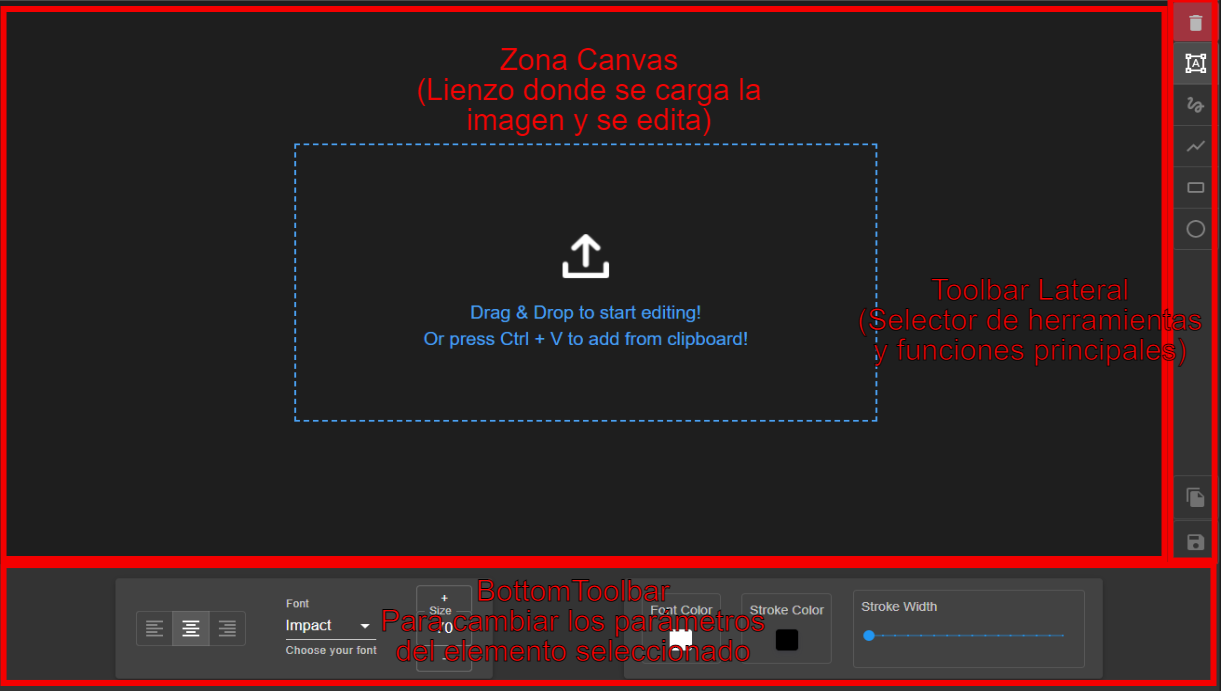
\includegraphics[scale=0.30]{img/ESQUEMA_PARTES.png}
  \caption{Esquema de las principales partes de la aplicación}
\end{figure}

\newpage
La principal ventaja que tiene dividir la aplicación en estos subcomponentes es que desde
React, podemos re-renderizar cada uno de forma individual cuando lo necesitemos, de esta forma
no hay que renderizar toda la página cada vez que se cambia un simple selector, sólo la o las
partes necesarias, lo que mejora notablemente el rendimiento y da una experiencia mucho mas
fluida al usuario.
\\\\
Tras crear una base de placeholders que diferencien las distintas partes planificadas
de la aplicación, comenzamos con el desarrollo de las primeras carácterísticas 
partiendo de las primeras historias de usuario.

%Justificar por qué esa biblioteca y hablar un poco de ella
\section{Biblioteca de canvas para React: KonvaJS}
Para empezar a elaborar la aplicación, comenzamos por la funcionalidad más básica necesaria
cargar multimedia en el lienzo del editor, necesitamos una imagen para editar y por
ende se comenzó por crear esta funcionalidad.
\\
Ya se había elaborado una carga de imagen en las demos de la fase de planificación, 
puramente en html y javascript, empleando el elemento HTML Canvas, en estas demos 
se pudo comprobar que para la tarea que queríamos realizar manejar el elemento
canvas desde el DOM\cite{DOM} no era eficiente, ni aprovechaba todas las ventajas 
de React.
El elemento HTML canvas es un mero array de píxeles, no hay manera de diferenciar 
los objetos dibujados en el canvas una vez dibujados, son solo píxeles de otro color,
para hacer esto, tenemos que tener los objetos almacenados en memoria y actualizar el
canvas repintando todos los objetos cada vez que se modifica algo, esto no es una 
tarea fácil, ya que hay que gestionar entre otras cosas la frecuencia de actualización
del canvas (frames per second) y asegurarse de que el código es eficiente, ya que 
no es una tarea trivial en potencia de procesado necesaria.
Por ende y tras investigar las distintas posibilidades se decidió utilizar una 
biblioteca específica para gestionar el elemento canvas HTML para React, de este
modo, podemos aprovechar las carácterísticas de React y olvidarnos de gestionar 
la frecuencia de actualización del canvas, ya que la biblioteca lo repinta cada vez
que se hace un cambio, además de tener una forma unificada de instanciar los objetos
que estan pintados en el canvas, todos los objetos que se pintan son instancias de 
hijos de clases propias de la biblioteca o directamente son instancias de clase de la 
misma.
\\\\
Tras investigar y barajar varias opciones se terminó decidiendo elegir KonvaJS 
\cite{KonvaJS} como biblioteca, primero porque era específica de React
(aunque tiene versiones para Vue.js ) 
y segundo, porque contaba con clases y métodos bastante interesantes para una aplicación
como un editor, el resto de bibliotecas estaban mucho mas enfocadas a animaciones, sin 
embargo, KonvaJS permite mucha mas inteacción con el lienzo, que es lo principal en un
editor.
%Como funciona
\section{El Drag\&Drop principal}
%Lo primero que se empezó a hacer despues de poder añadir la imagen
Habiendo importado las dependencias necesarias para KonvaJS\cite{KonvaJS} en el proyecto,
se comenzó a implementar la funcionalidad mas básica y necesaria del editor, para editar,
necesitamos tener algo que editar. 
\\
En este punto había que tener en cuenta una de las principales intenciones del proyecto,
se debía poder utilizar el editor sin necesidad de descargar nada o utilizar archivos
guardados en la memoria local, es decir, que había que poder añadir contenido desde 
el portapapeles al editor, aunque también se da la opción de usar contenido local.
\\
Para comenzar, se creó un componente de React que se renderizaría cuando no haya 
nada cargado en el lienzo.

\begin{lstlisting}[caption={Renderizado condicional del componente del DragandDrop}]
  {//If there is no image, show draganddrop input
  ( this.state.image == null ) ?
      <DragandDrop imgLoader={this.imageLoader.bind(this)}/> 
      : 
      <SecondaryDragandDrop 
          imgLoader={this.createNewSecondaryImage.bind(this)}
      />
  }
\end{lstlisting}

Este componente consiste en un área de drop donde el usuario puede añadir el archivo 
haciendo drag desde su PC, se emplea el evento OnDrop para leer el fichero, si es
del formato correcto, se lee y se manda al componente padre (editor) para cargarlo en 
el canvas.
\\
El canvas se carga haciendo uso de la biblioteca KonvaJS \cite{KonvaJS}, desde React 
no tenemos un elemento canvas, tenemos el componente Stage de la biblioteca, así que 
lo cargamos en él, haciendo uso de los métodos de la biblioteca.
\\\\
El canvas se renderiza desde el principio de la aplicación, al principio se pensó 
en hacer un renderizado condicional al igual que con la zona de drop, pero el Stage
(el canvas en el DOM), es el elemento más importante de toda la aplicación
que además es necesario para el funcionamiento base de la propia aplicación 
(no se puede editar nada sin él, es el propio lienzo), así que no tenía mucho sentido
condicionar su renderizado ya que no aportaba nada,
para evitar posibles complicaciones simplemente se renderiza en oculto con ancho y alto
de 0.
\\\\
Cuando se carga una nueva imagen necesitamos calcular qué tamaño tendrá el lienzo, 
cada imagen puede tener un tamaño completamente diferente y queremos que la aplicación
tenga consistencia, es decir, que el usuario sienta que siempre tiene un área de edición
parecida independientemente de la resolución de la imagen.
Para ello debemos tener dos cosas en cuenta, el tamaño de la zona de edición del usuario,
que depende de su propia pantalla y el tamaño original de la imagen.
La correlación de la imagen siempre habrá que mantenerla para que no se deforme la 
imagen base, la calculamos y manteniendo esa correlación ajustamos la imagen al tamaño
disponible dejando algo de espacio por estética (para las imágenes demasiado pequeñas, 
no se efectua ajuste porque no es necesario).

\begin{lstlisting}[caption={Método para calcular el tamaño del lienzo a partir de una imagen}]
  calculate_resize(correlation, width, height){
        let pixel_margin = 100
        //wide photo
        if( correlation <= 1 ){
            //image too small, dont correct
            width = (width > 400 ? width - pixel_margin : width)
            //
            if( correlation * width < height ){
                height = (correlation * width) - pixel_margin
                width = width - pixel_margin
            } else {
                width = height * (1/correlation) - pixel_margin
                height = height - pixel_margin
            }

        //long photo
        } else {
            //image too small
            height = (height > 400 ? height - pixel_margin : height)
            //
            if( height * (1/correlation) < width ){
                width = height * (1/correlation)
                //height = height
            } else {
                width = width - pixel_margin
                height = correlation * width - pixel_margin
            }
        }

        return {
            width: width,
            height: height
        }
    }
\end{lstlisting}

\section{La primera herramienta: Añadir Texto}
Ya que tenemos el mínimo necesario, que es tener una imagen que empezar a modificar, 
comenzamos a implementar la primera funcionalidad, al ser un editor especialmente
enfocado en facilitar la edición de memes, se comenzó por la funcionalidad mas básica
para hacer un meme, el texto, 

\section{Cambio de propiedades: BottomToolbar}
%Fusion de creación de texto con el selector

\section{Cambio entre herramientas: Toolbar}
%Como funciona el componente bottomtoolbar y como va cambiando
%Comentar aquí todo el tema handlers, updates etc y como se sincroniza
%con el cambio de item, es igual para todas las herramientas

\section{Herramienta: Selector}
\section{Herramienta: Lineas}
  \subsection{Herramienta Freeline}
  \subsection{Herramienta StraghtLine}
\section{Herramienta: Formas Geométricas}
  \subsection{Herramienta: Rectángulos}
  \subsection{Herramienta: Elipses}
\section{Herramienta: Imágenes superpuestas}
Como no podía faltar en un editor de memes

%konva

\iffalse
Esquema para luego redactar bien:
- A partir de la demo rehice todo para adaptarlo a la libería 

- Lo primero fue hacer que se pudiera añadir una foto base (DragAndDrop y Konva canvas)

- Explicar todo tema lienzo, cálculos etc..

- Se añadió poder quitar la foto y volver a añadir otra

- Comenzamos el poder añadir texto

- todo tema texto, textarea, propiedades, drag, transformador, lo de adaptar el texto al tamaño de la caja bla bla 

- Comienzo de la toolbar para poder poner el texto bonito

- Tema toolbar, material-ui, como mandamos la info desde la toolbar al texto y lo actualizamos bla bla

- Hablar de ajustes varios, tema eventos etc.. clicks handlers bla bla

- Añadido el ctrl + v de imagen principal (esto quizá explicarlo después para juntar todo el tema texto)

- Handleo de varios textos diferentes

- Cuando ya se cambiaban los textos desde la toolbar ahora como se cambia la toolbar para que coincida con las opciones del texto

- Hablar un poco de tema componentes funcionales vs clases (todos los cambios que se hicieron)

- PRIMERA TANDA DE TESTS (preguntar a JJ si explicar esto todo luego o aquí)

- Además de texto ahora a añadir mas cosas, Imágenes y sus transformaciones

- Hablar del tema lineas, como se movian las cosas al pintar encima, la lógica de las herramientas
  como se ha solucionado, porque se ha hecho así y el React.clone()

- [pensar lo que falta por aqui]

- tema eventos, copiar pegar, guardar etc

-production build

-despliegue

\fi

\newpage
\section{Tests}

Como es costumbre en las metodologías ágiles, se ha testeado, en la medida de lo posible,
todo el código que se ha ido desarrollando según se iba añadiendo a la aplicación.
Para ello necesitabamos escoger de que manera íbamos a testear nuestro código, se barajaron
varias opciones, como el módulo de tests-utils que trae react-dom \cite{react-dom} o jest, 
pero estos módulos no encajan lo suficientemente bien con una aplicación como un editor, 
algo que es muy interactivo y gráfico requería testearlo también de forma gráfica. Por ende
se terminó escogiendo Cypress \cite{cypress} que es una herramienta que simula un navegador de
forma gráfica y genera los eventos, además cuenta con un módulo para React \cite{cypressReact} que permite montar
y testear componentes individualmente, además de comprobar el estado (state) de React, cosa
que no permiten la mayoría de aplicaciones de testeo gráfico, ya que, en el navegador los
componentes no existen como tal, sólo el código HTML que genera React a partir de estos.

\begin{figure}[!h]
  \centering
  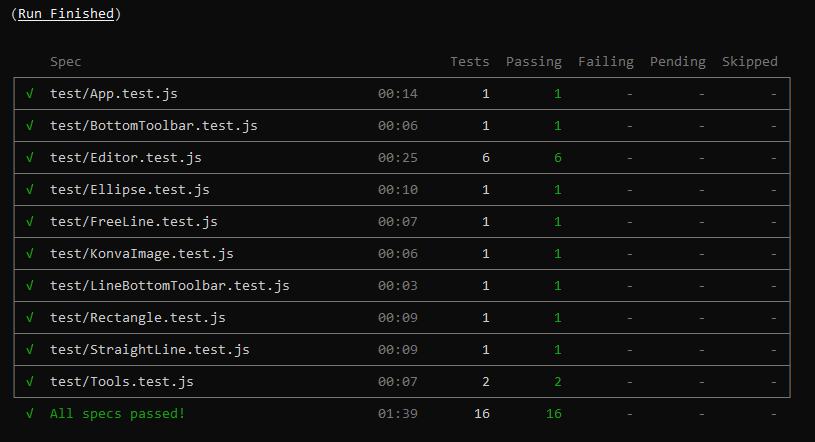
\includegraphics[scale=0.6]{img/TestsOK.png}
  \caption{Resultado de la ejecución de los tests de cypress, run-ct}
\end{figure}

Lo ideal es testear el 100\% del código de la aplicación, aunque en la realidad llegar a esto
es bastante complicado, se ha intentado cubrir la mayor parte posible, para ello se han creado
tests para cada historia de usuario que hemos definido, crear el test era requisito para considerar
terminada la historia de usuario y como es lógico el test debía testear la funcionalidad que 
proponía la HU. Hubo una excepción en las primeras historias de usuario que se completaron
no se testearon directamente, ya que el testeo se comenzó algo mas tarde para esperar a 
que la aplicación tuviera ciertas funcionalidades básicas completas ya que en el inicio es
muy fácil que ciertas partes cambien drásticamente y así evitar rehacer tests de forma innecesaria,
de todos modos, estas partes fueron testeadas en cuando se empezaron a desarrollar los tests.

\newpage
\section{Despliegue de la aplicación}

Ahora solo nos falta desplegar la aplicación, en nuestro caso se va a desplegar esta primera 
versión utilizando el servicio de Github Pages \cite{GithubPages}.
\\
Como comentamos al inicio, para crear esta aplicación empleamos el paquete create-react-app \cite{create-react-app},
este paquete cuenta con scripts que ayudan en el despliegue de la aplicación y crean una 
versión optimizada del código.
Como era uno de los objetivos del desarrollo, la aplicación ha sido desarrollada pensando
en hacer que, aunque sea una aplicación multimedia, no se requiera de un servidor potente que
soporte mucha carga, es decir, es puro front-end, así que sólo necesitamos que el servidor
envíe código HTML, CSS y los scripts de Javascript, no tiene que procesar nada relativo a las
ediciones que haga el usuario ya que esas operaciones se efectuan en el cliente.
\\
Esto nos permite emplear hostings ligeros para el despligue, 
%en nuestro caso hemos decidido
%emplear Github Pages por 3 razones, el proyecto ya estaba siendo desarrollado en Github,
%el paquete create-react-app \cite{create-react-app} tiene soporte para Github Pages \cite{GithubPages}
%y por qué no decirlo, es gratuito y funciona bastante bien.
los hostings mas usados son Azure, Firebase o AWS aunque son bastante flexibles son hostings 
bastante potentes y de pago, gracias a como está construida la aplicación no necesitamos tanto,
así que vamos a emplear Github Pages por varias razones, el paquete 
create-react-app \cite{create-react-app} tiene soporte para Github Pages \cite{GithubPages}
y por qué no decirlo, es gratuito y funciona bastante bien.
\\
Para el despliegue se han seguido las instrucciones que nos da la documentación de 
create-react-app para hacer deploy en Github Pages \cite{GithubPagesDeploy}.
Es bastante simple, añadimos la configuración de la ruta donde se hará el deploy e instalamos
el paquete npm gh-pages \cite{gh-pages}, que es el que recomienda la documentación oficial.
Y añadimos unos scripts que hacen uso del paquete para el deploy, al ejecutar el script
crea una branch que sirve como source estático de la web.
\\\\
El despliegue puede probarse en el siguiente enlace: \url{https://bytevictor.github.io/memeHub/}